\documentclass[a4paper, 12pt]{article}


\usepackage[french]{babel}
\usepackage[utf8]{inputenc}
\usepackage[T1]{fontenc}
\usepackage{lmodern}
\usepackage{listings}
\usepackage{graphicx}
\usepackage{amsmath}
\usepackage{amsfonts}
\usepackage{amssymb}
\usepackage{caption}
\usepackage{subcaption}
\usepackage[usenames,dvipsnames]{xcolor}


\setcounter{secnumdepth}{4}
% TAILLE DES PAGES (A4 serré)

\setlength{\parindent}{0pt}
\setlength{\parskip}{1ex}
\setlength{\textwidth}{17cm}
\setlength{\textheight}{24cm}
\setlength{\oddsidemargin}{-.7cm}
\setlength{\evensidemargin}{-.7cm}
\setlength{\topmargin}{-.5in}

% Commandes de mise en page
\newcommand{\fichier}[1]{\emph{#1}}
\newcommand{\nom}[1]{\emph{#1}}
\newcommand{\Fig}[1]{Fig \ref{#1} p. \pageref{#1}}
\newcommand{\itemi}{\item[$\bullet$]}

% Commandes de maths
\newcommand{\fonction}[3]{#1 : #2 \to #3}
\newcommand{\intr}[2]{\left[ #1 ; #2 \right]}
\newcommand{\intn}[2]{\left[\![ #1 ; #2 \right]\!]}
\newcommand{\intro}[2]{\left] #1 ; #2 \right[}
\newcommand{\intrsod}[2]{\left[ #1 ; #2 \right[}
\newcommand{\ps}[2]{\langle #1, #2 \rangle}
\newcommand{\mdelta}[1]{\boldsymbol{\delta_{#1}}}
%% \newcommand{\mdelta}[1]{\delta_{\textbf{#1}}}

\pagenumbering{arabic}
\graphicspath{{images/}}

\title{ASM-TP2 : ACP-régression en génétique} 
\author{Pierre Petitbon \and Florian Privé \and Xinrui Xu}
\date{}

\begin{document}

\maketitle

\section{Préparation des données}

\begin{enumerate}
\setlength{\itemsep}{20pt}

\item[1.a)] 
\item[1.b)] 
Le script place toutes les origines des individus des données sur une carte du continent américain, suivant la latitude et la longitude. La carte obtenue correspond bien à celle du sujet. 
\end{enumerate}



\section{Régression}
Le problème c'est qu'on est incapable de trouver les coefficients de la régression de la longitude car le nombre de marqueurs génétiques (5709) est beaucoup plus grand que le nombre d'individus (494). C'est pourquoi on régressera la latitude et la longitude avec les scores de l'ACP faite les marqueurs génétiques. 

À refaire (avec le cours) avec une démonstration mathématique.

\section{ACP}
\begin{enumerate}
\setlength{\itemsep}{20pt}
\item[3.a)]
 L'analyse en composantes principales consiste à transformer des variables corrélées en nouvelles variables décorrélées les unes des autres. Ces nouvelles variables sont appelées composantes principales. Elle permet de faire une analyse sur moins de variables et réduit la redondance de l'information. 

 \item[3.b)]
 On réalise une ACP sur les données génétiques avec tous les individus.

\end{enumerate}


\section{Sélection du meilleur sous-ensemble. Méthode «Best subscript selection»}

\begin{enumerate}
\setlength{\itemsep}{12pt}

\item[4.a)] On ne peut se limiter à l'analyse du modèle en partie 2 car on garde tous les paramètres sans distinction. Il faudrait ne garder que les prédicteurs pertinents, qui ont une influence réelle sur lcavol. Certains prédicteurs ne servent qu'à approcher le bruit dans l'échantillon, ce qui permet effectivement de se rapprocher des données, mais cela dégrade la qualité des prédictions. On parle alors d'overfitting.

Autrement dit, le problème majeur est que le critère RSS est insuffisant : plus on a de prédicteurs, meilleure la régression est jugée. Or, les prédictions peuvent se détériorer lorsqu'on utilise des prédicteurs superflus qui ne servent qu'à approcher le bruit.

\item[4.b)] Pour chaque $k$ dans $\{0, ..., 8\}$, on fait varier le choix des prédicteurs afin de minimiser le RSS. La courbe des RSS ainsi obtenus vérifie bien la décroissance avec le nombre de prédicteurs. On observe un saut important à l'ajout du premier prédicteur (le RSS diminue de moitié), ce qui n'a rien d'étonnant : cela témoigne de l'intérêt de faire une régression. A l'ajout du deuxième puis du troisième prédicteur, le RSS diminue encore assez significativement, puis il reste presque inchangé au-delà.

\begin{figure}
\begin{center}
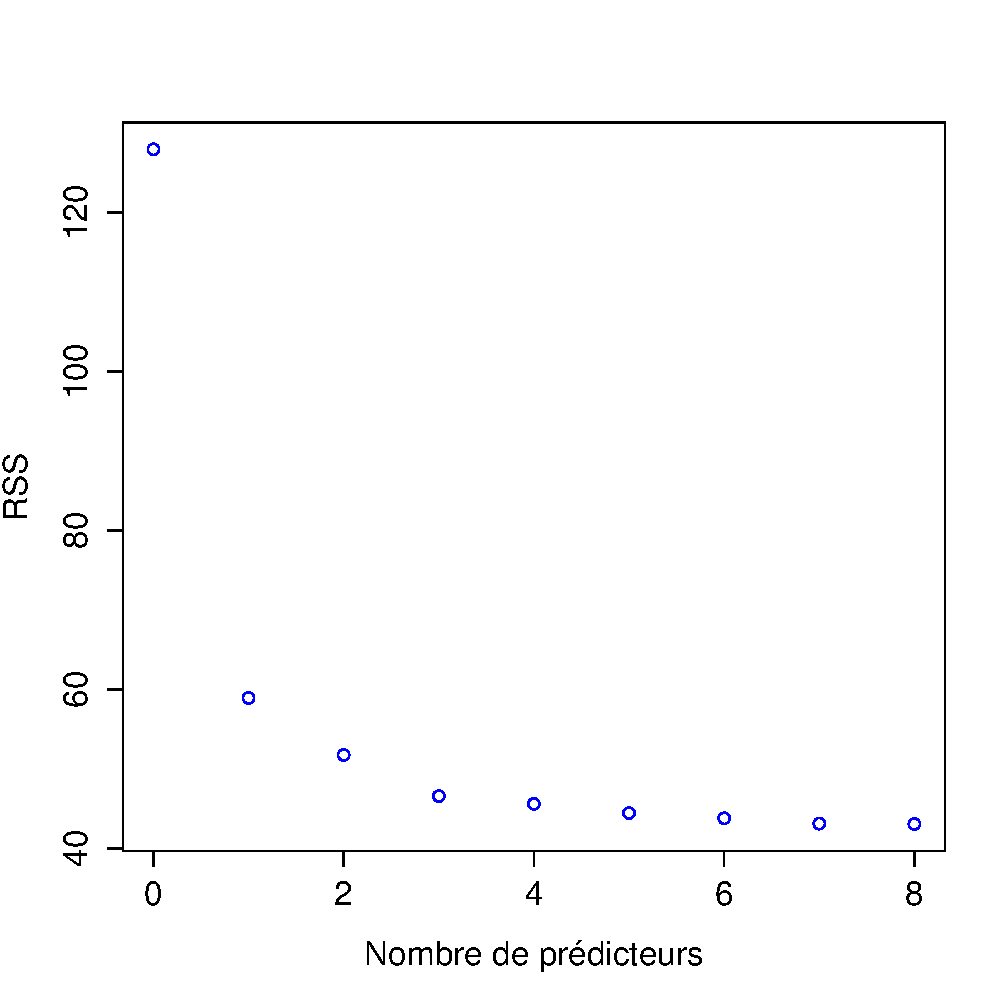
\includegraphics[scale=1]{rss.pdf}
\caption{Graphe des RSS en fonction du nombre de prédicteurs}
\end{center}
\end{figure}

On indique ci-dessous les sous-ensembles de prédicteurs qui réalisent le minimum de RSS, à nombre de prédicteurs $k$ fixé :
\begin{itemize}
\item $k = 0: \emptyset$
\item $k = 1: \{lcavol\}$
\item $k = 2: \{lcavol, lweight\}$
\item $k = 3: \{lcavol, lweigth, svi\}$
\item $k = 4: \{lcavol, lweight, lbph, svi\}$
\item $k = 5: \{lcavol, lweight, age, lbph, svi\}$
\item $k = 6: \{lcavol, lweight, age, lbph, svi, lcp\}$
\item $k = 7: \{lcavol, lweight, age, lbph, svi, lcp, pgg45\}$
\item $k = 8: \{lcavol, lweight, age, lbph, svi, lcp, gleason, pgg45\}$
\end{itemize}

\item[4.c)] Cette méthode ne permet pas de sélectionner le meilleur modèle, toutes tailles confondues, il ne permet que de déterminer le modèle qui "colle" le plus aux données, le nombre de prédicteurs étant fixé. Le meilleur modèle n'est pas nécessairement celui qui considère le plus de prédicteurs. En particulier, on n'évalue toujours pas la qualité des prédictions, qui est le seul critère qui importe véritablement. L'objectif de la split-validation est justement de tenir compte de ce critère pour affiner le choix du modèle.

\end{enumerate}


\section{Split-validation}

\begin{enumerate}
\setlength{\itemsep}{20pt}

\item[5.a)] La split-validation consiste à séparer les échantillons en deux sous-ensembles :

\begin{itemize}
\item Une partie pour effectuer différentes régressions (ensemble d'apprentissage)
\item Une partie pour tester les différents modèles de régression possibles, et sélectionner celui qui produit les meilleures prédictions (ensemble de test)
L'ensemble de test permet donc de comparer les valeurs prédites aux valeurs mesurées.
\end{itemize}

\item[5.c)] Le meilleur modèle de taille 2 contient les prédicteurs $i = 1$ (lcavol) et $j = 2$ (lweight). lm(lpsa~.,data=pro[-valid,c(i,j,9)]) correspond au calcul de la régression sur l'ensemble d'apprentissage (-valid), en s'intéressant uniquement aux prédicteurs lcavol et lweight.

L'erreur d'apprentissage moyenne pour ce modèle est $0.503$. A noter que l'erreur est prise au sens des moindres carrés.

\item[5.d)] L'erreur de prédiction moyenne est $0.575$. On peut observer qu'elle est du même ordre de grandeur que l'erreur d'apprentissage moyenne.

\item[5.e)] En se basant sur cette unique split-validation, nous prendrions le modèle avec 2 prédicteurs. En effet, il s'agit du modèle qui minimise l'erreur de prédiction (cf. figure 3), qui est à nos yeux le critère essentiel pour juger d'un modèle de régression. Les deux prédicteurs retenus sont lcavol et lweight.

\item[5.f)] Le principal problème de la méthode de split-validation est la séparation arbitraire de l'échantillon en un ensemble d'apprentissage et un ensemble de test. Les résultats de la split-validation sont sensibles à cette séparation. En optant pour une séparation aléatoire des échantillons, la split-validation indique cette fois-ci qu'il faudrait prendre le modèle avec 3 prédicteurs car c'est à présent celui qui minimise l'erreur de prédiction (cf. figure 4).

\item[5.g)] Pour éviter ce problème, nous proposons d'itérer un nombre donné de fois (30 dans notre script) l'algorithme de split-validation avec séparation aléatoire de l'échantillon en deux moitiés de même taille. On récupère alors pour chaque itération les erreurs d'apprentissage et de prédiction moyennes. On calcule alors la moyenne de ces erreurs, et on se base sur ces résultats pour tirer des conclusions quant au choix du modèle. Les variations d'une itération à l'autre sont ainsi gommées. Avec cette méthode, on obtient que le meilleur modèle est celui avec 3 prédicteurs (cf figure 5).



\end{enumerate}


\section{Conclusion}

D'après notre analyse, le meilleur modèle prédictif pour lpsa est le modèle de régression à 3 prédicteurs $\{lcavol, lweigth, svi\}$. 
Chacun de ces prédicteurs est corrélé positivement avec lpsa avec une probabilité d'erreur très faible (On note $P_{e}$ cette probabilité d'erreur).

Attardons-nous sur chacun de ces prédicteurs :

\begin{description}
\item[lcavol :] log volume de cancer. Corrélation très sûre ($P_e = 3.49*10^{-10}$) avec lpsa. Ce résultat confirme le fait que les cellules prostatiques cancéreuses sécrètent dix fois plus de lpsa que les cellules normales.
\item[lweight :] log poids de la prostate. Corrélation très sûre ($P_e = 0.0289 \%$) avec lpsa. Ce résultat est cohérent lui aussi : étant donné que toutes les cellules prostatiques (cancéreuses ou non) sécrètent du lpsa, une prostate plus lourde signifie plus de cellules prostatiques, donc plus de sécrétions de lpsa.
\item[svi :] invasion de la vésicule séminale. Corrélation sûre ($P_e = 0.180 \%$). La quantité de cellules cancéreuses dans la vésicule séminale semblent être corrélée positivement à la sécrétion de lpsa. On peut conjecturer que $svi = f(cavol)$, où cavol est le volume de cancer, et f est une fonction non logarithmique. Svi apparaîtrait alors comme un prédicteur supplémentaire qui permet d'affiner l'interpolation, mais surtout d'améliorer les prédictions.
\end{description}

\begin{figure}
\begin{center}
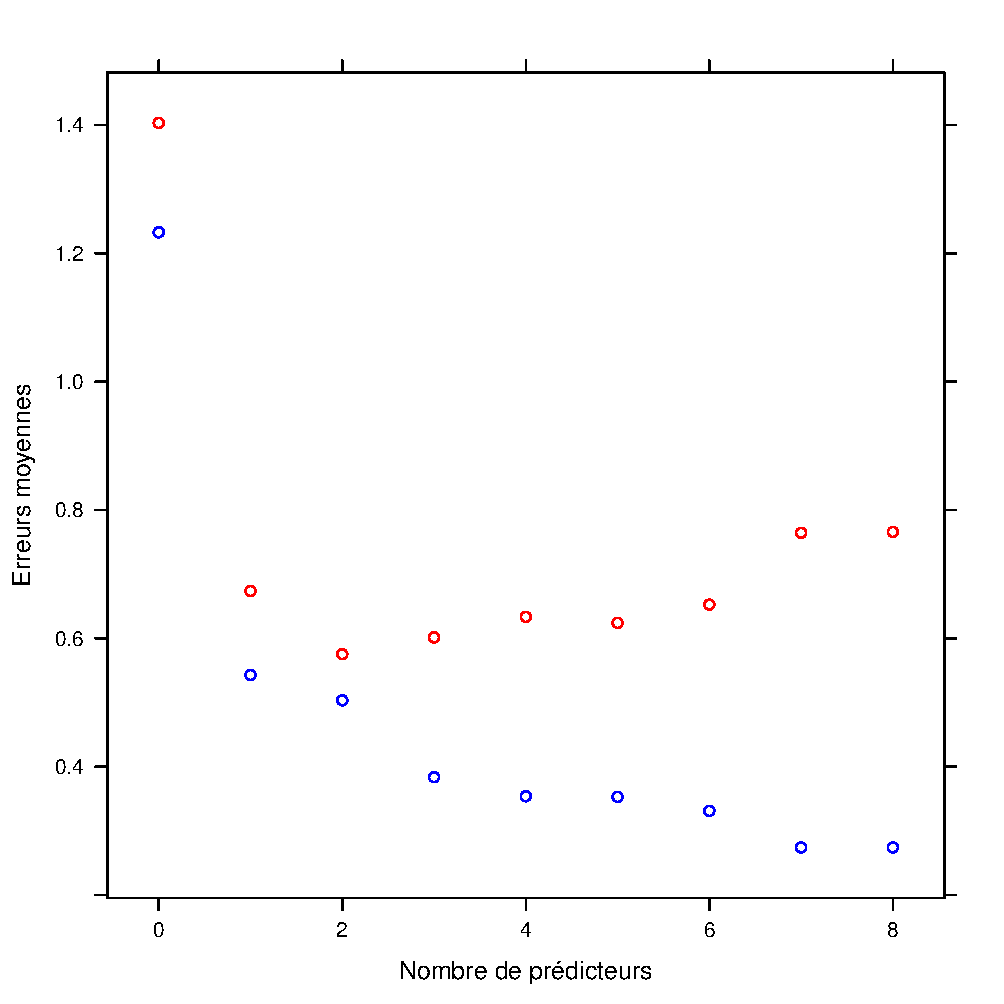
\includegraphics[scale=1]{erreurs_moy.pdf}
\caption{Tracé des erreurs d'apprentissage (en bleu) et de prédiction (en rouge) moyennes en fonction du nombre de prédicteurs}
\end{center}
\end{figure}

\begin{figure}
\begin{center}
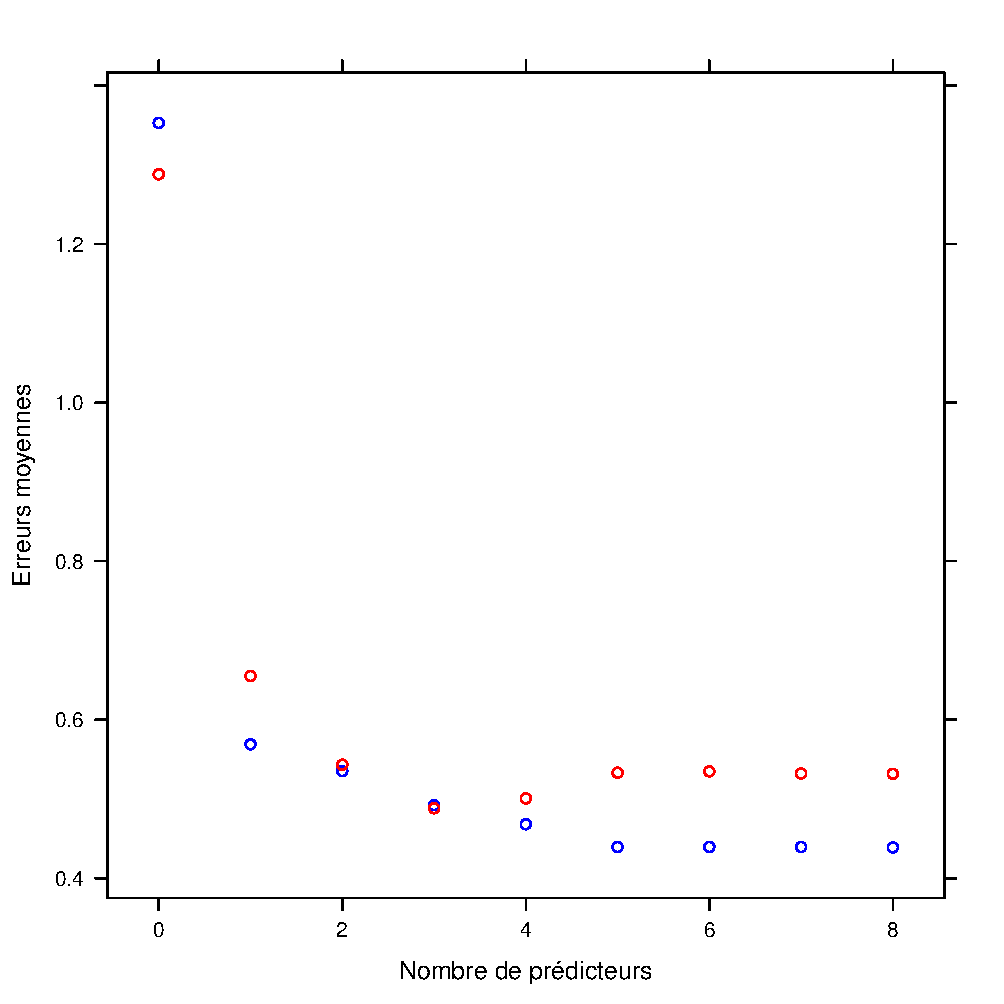
\includegraphics[scale=1]{erreurs_moy_autre.pdf}
\caption{Tracé des erreurs d'apprentissage (en bleu) et de prédiction (en rouge) moyennes pour une séparation aléatoire de l'échantillon}
\end{center}
\end{figure}

\begin{figure}
\begin{center}
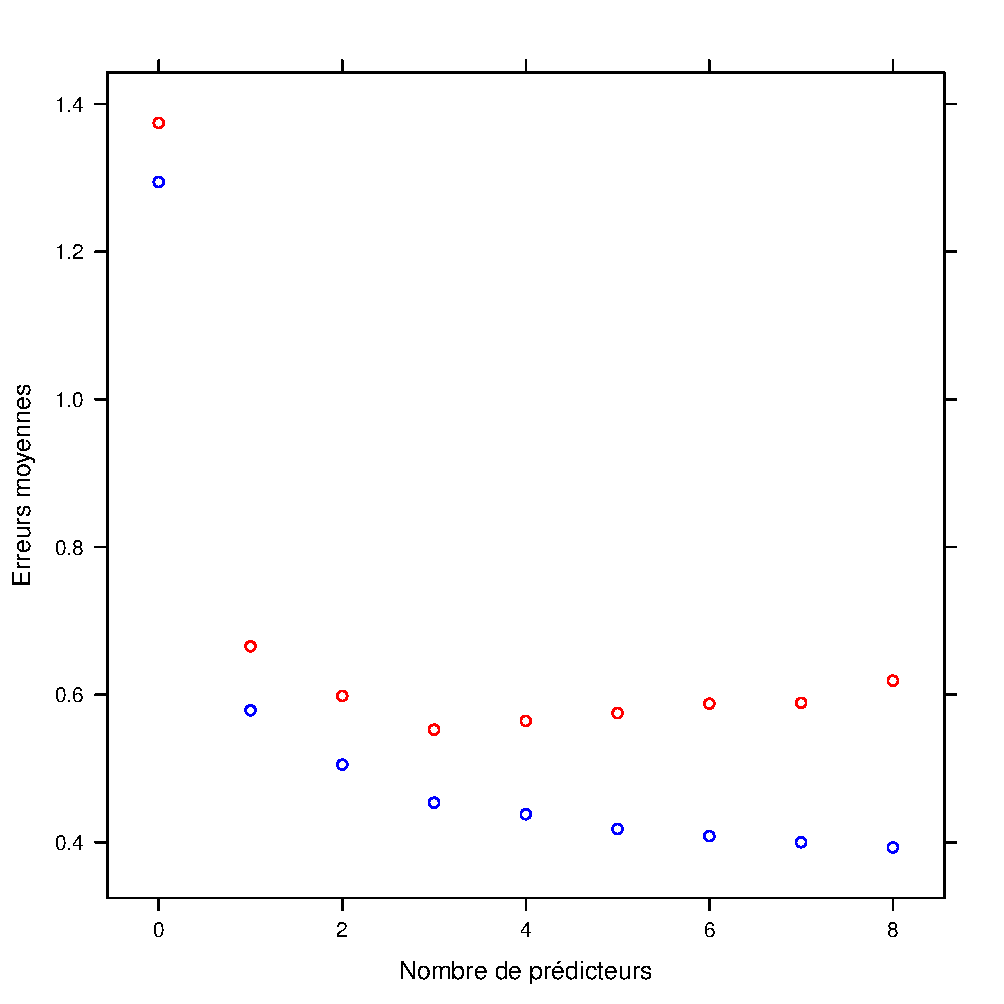
\includegraphics[scale=1]{erreurs_moy_moy.pdf}
\caption{Tracé des erreurs d'apprentissage (en bleu) et de prédiction (en rouge) moyennes sur 30 itérations avec séparation aléatoire}
\end{center}
\end{figure}

\end{document}

% TODO : parler du scrum master
